\section{梯度的处理}
\label{sec:sgdb-processing}

前两节的方向都由读数线性组合或缩放而来。本节研究更直接的改动：读数被截短、用有限精度算出、来自过去的点，甚至换成一个人为规定的向量。这些操作都使实际方向偏离原目标的梯度。

实际方向在什么点上、以什么误差近似当前梯度，这个误差怎样影响原目标上的进展？回答时把实际读数分解成三部分：真梯度$\bm{g}^{(t)}$、由历史确定的条件偏差$\bm{b}^{(t)}$、零条件均值的噪声$\bm{\xi}^{(t)}$，
\begin{equation}
 \hat{\bm g}^{(t)}=\bm{g}^{(t)}+\bm{b}^{(t)}+\bm{\xi}^{(t)},\qquad
 \mathbb{E}\bigl[\bm{\xi}^{(t)}\mid\mathcal{F}^{(t)}\bigr]=\bm{0}.
 \label{eq:sgdb-reading-decomposition}
\end{equation}

这个分解在前面的读数误差分析中已经用过，这里偏差项不再为零。下面分别看裁剪、近似和替代三种情形下$\bm{b}^{(t)}$从哪里来、能否被控制。

\subsection{梯度裁剪}
\label{sec:sgdb-clipping}

\paragraph{两种裁剪}
\term{梯度裁剪}（gradient clipping）在读数过大时把它截短，防止个别很大的读数把参数推得太远\scite{pascanu2013}。给定阈值$c>0$，有两种做法。\term{逐坐标裁剪}（coordinate-wise clipping）把每个坐标截到$[-c,c]$内：
\begin{equation}
 \bigl[\operatorname{clip}^{\mathrm{co}}_c(\bm{g})\bigr]_j=\max\{-c,\min\{c,g_j\}\}.
 \label{eq:sgdb-clip-coord}
\end{equation}

\term{范数裁剪}（norm clipping）整体缩放，只在范数超过阈值时起作用：
\begin{equation}
 \operatorname{clip}_c(\bm{g})=\bm{g}\cdot\min\Bigl\{1,\frac{c}{\lVert\bm{g}\rVert_2}\Bigr\}.
 \label{eq:sgdb-clip-norm}
\end{equation}

下面用同一个读数比较。取$\bm{g}=(3,4)$，$c=1$，两种裁剪的结果是
\[
 \operatorname{clip}^{\mathrm{co}}_1(\bm{g})=(1,1),\qquad
 \operatorname{clip}_1(\bm{g})=(0.6,0.8).
\]

前者的范数是$\sqrt2$，方向从与第一坐标轴夹角约$53^\circ$变成$45^\circ$；后者的范数是$1$，方向不变。图~\ref{fig:sgdb-clip-bias}(a)表明，逐坐标裁剪是投影到边长$2c$的正方形，范数裁剪是投影到半径$c$的圆盘。

\begin{BookInlineFigure}
  \centering
  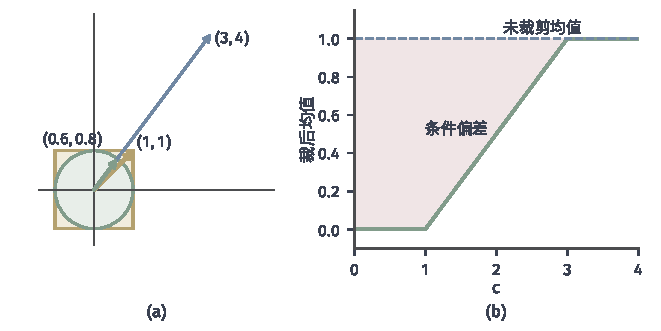
\includegraphics[width=112mm]{figures/05-optimization/05-stochastic-optimization/matplotlib/sgdb-clip-bias/figure.pdf}
  \caption{裁剪的几何与偏差。(a)读数$(3,4)$（蓝）在$c=1$时的两种裁剪：逐坐标裁剪得到黄色正方形角上的$(1,1)$；范数裁剪沿原方向缩到绿色圆上的$(0.6,0.8)$。(b)读数以相等概率取$3$或$-1$，绿线是逐点裁剪后的均值关于阈值$c$的变化，蓝色虚线是未裁剪的均值$1$，红色区域是两者之差。}
  \label{fig:sgdb-clip-bias}
\end{BookInlineFigure}

\paragraph{裁剪放在哪里}
一个算法中可以裁剪的位置不止一处，图~\ref{fig:sgdb-clip-position}标出了四处。裁剪位置$1$：裁剪逐样本读数后再平均，后面的动量和统计看到的都是裁过的量。裁剪位置$2$：先平均再裁剪批量读数。裁剪位置$3$：裁剪动量方向，统计仍记录原始读数。裁剪位置$4$：裁剪缩放后的方向，也就是最终的位移。

\begin{BookInlineFigure}
  \centering
  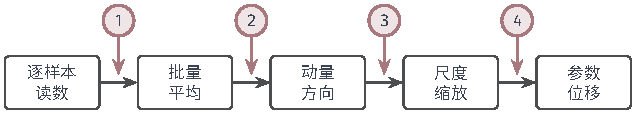
\includegraphics[width=107.64mm]{figures/05-optimization/05-stochastic-optimization/tikz/sgdb-clip-position/figure.pdf}
  \caption{更新流水线上可以施加裁剪的四个位置，圆圈内的数字对应正文的编号。位置不同，得到的是不同的算法，描述一次运行时要写明位置和阈值。}
  \label{fig:sgdb-clip-position}
\end{BookInlineFigure}

位置$1$和位置$2$的差别，用贯穿例在$x=2$处的三项读数说明。取$c=2$，全批量读数$5,4,-3$。先逐项裁剪再平均，得到
\[
 \frac13\bigl(2+2-2\bigr)=\frac23.
\]
先平均再裁剪，平均是$f'(2)=2$，未超过阈值，裁剪不起作用，得到$2$。前者有偏差，后者这里没有。

增大批量能否减小偏差，也取决于位置。逐样本裁剪后再平均，批量越大，平均越接近裁后读数的均值，偏差不随批量变小。先平均再裁剪时，批量越大，平均读数越集中在真梯度附近，只要真梯度的范数小于阈值，被裁剪的概率就越小，偏差随之减小。

\paragraph{用两点分布核对偏差}
裁剪是非线性运算，它改变读数的平均。设读数以相等概率取$3$与$-1$，均值为$1$。用$c=1$裁剪后，读数变为$1$与$-1$，均值为$0$：
\[
 \mathbb{E}\bigl[\operatorname{clip}_1(\hat g)\bigr]=0\neq1.
\]

条件偏差是$-1$，等于真梯度的相反数，方向信息完全消失。图~\ref{fig:sgdb-clip-bias}(b)画出裁后均值随阈值的变化：$c<1$时为$0$，$1\leq c<3$时为$(c-1)/2$，$c\geq3$时才恢复为$1$。

所以裁后的读数不能当作无偏梯度套用前面的定理。贯穿例能说明后果。取$c=2$的逐项裁剪，期望方向在$x=0$处为
\[
 \frac13\bigl(\operatorname{clip}_2(3)+\operatorname{clip}_2(0)+\operatorname{clip}_2(-9)\bigr)=\frac13(2+0-2)=0.
\]
也就是说，逐项裁剪的均值在$x=0$处恰好为零，而真正的最优点是$x^\star=1$，$f(0)-f^\star=1$。裁剪把期望更新的平衡点从$x=1$移到了$x=0$。

\paragraph{分别评价两种作用}
裁剪的作用要分开评价。第一是控制位移：范数裁剪在位置$2$或位置$4$保证每步位移的范数不超过$\alpha c$，这是确定的。第二是控制二阶矩：裁后读数的范数不超过$c$，所以它的二阶矩不超过$c^2$。原读数的二阶矩很大甚至无穷时，裁剪之后前面依赖方差假设的分析才可能使用。

这两种好处的代价是偏差$\bm{b}^{(t)}$。偏差怎样影响进展，由下一小节的递推回答。是否值得用偏差换取有界的二阶矩，要看具体的读数分布，没有无条件的结论。

\subsection{近似梯度}
\label{sec:sgdb-approximate}

\paragraph{几种来源}
实际得到的方向常常不是当前点的精确读数。下面三种情形都先问两件事：方向在哪个求值点上计算，误差能否由计算预算或步长控制。

第一是有限精度。例如浮点运算或内层线性方程只解到某个残差，读到的是$\nabla f(\bm{x}^{(t)})$的近似，误差$\bm{b}^{(t)}$的大小由内层的求解精度决定，增加每步计算可以使它变小。第二是量化，把读数的每个分量化到间距$\Delta$的格点上，$\lvert b_j\rvert\leq\Delta/2$，这是确定的偏差。真梯度比半个格子还小时，量化后的读数恰好是零，迭代会停在一个有残差的点上。第三是延迟读取，在第$t$轮用$\tau$轮之前的点上的梯度$\nabla f(\bm{x}^{(t-\tau)})$，也就是求值点不是当前点。

延迟的误差由步长控制，但可能破坏稳定性。设$f(x)=\frac12x^2$，用延迟$\tau=1$的精确梯度，
\[
 x^{(t+1)}=x^{(t)}-\alpha x^{(t-1)}.
\]
特征方程是$r^2-r+\alpha=0$。当$\alpha\in(0,1)$时，两根的模都小于$1$：两根为实数时积为$\alpha$，和为$1$，都在$(0,1)$内；两根共轭时模的平方等于积$\alpha$。当$\alpha=1$时两根落在单位圆上，迭代恰好以周期$6$循环。没有延迟时，$\alpha$可以取到$2$，所以延迟把稳定的步长范围缩小了一半。图~\ref{fig:sgdb-bias-delay}(b)是$\alpha=1$的情形，$\tau=2$时发散。

\begin{BookInlineFigure}
  \centering
  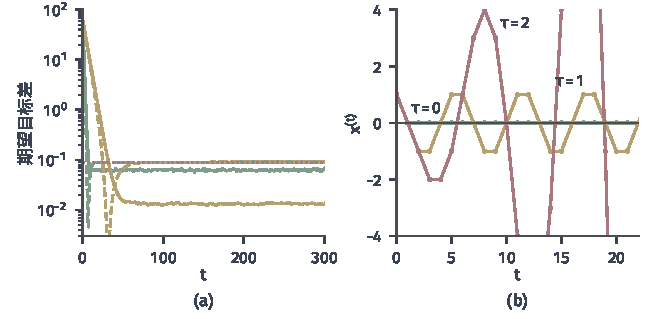
\includegraphics[width=112mm]{figures/05-optimization/05-stochastic-optimization/matplotlib/sgdb-bias-delay/figure.pdf}
  \caption{偏差、噪声与延迟的影响。(a)目标$f(x)=(x-1)^2+5$，初值$x=9$，$2000$次独立运行的平均目标差，绿线$\alpha=0.2$，黄线$\alpha=0.05$。实线是只有方差为$1$的噪声；虚线是只有常数偏差$b=0.6$，两种步长最终都停在红色点线$b^2/4=0.09$上。(b)目标$\frac12x^2$，$\alpha=1$，延迟$\tau=0,1,2$的迭代点。}
  \label{fig:sgdb-bias-delay}
\end{BookInlineFigure}

\paragraph{把偏差和噪声代入递推}
现在按式~\eqref{eq:sgdb-reading-decomposition}把两类误差代入有限步递推。下面的结果与前面的无偏分析结构相同，只多了偏差产生的一项。

\begin{theorem}[有偏读数下的平均平方梯度范数]
\label{thm:sgdb-biased}
设$f$梯度$L$-Lipschitz连续，下确界为$f_{\inf}$。设读数满足式~\eqref{eq:sgdb-reading-decomposition}，其中$\bm{b}^{(t)}$由$\mathcal{F}^{(t)}$确定，并且
\begin{equation}
 \lVert\bm{b}^{(t)}\rVert_2\leq B,\qquad
 \mathbb{E}\bigl[\lVert\bm{\xi}^{(t)}\rVert_2^2\mid\mathcal{F}^{(t)}\bigr]\leq\sigma^2 .
 \label{eq:sgdb-biased-condition}
\end{equation}
取固定步长$0<\alpha\leq1/L$，用$\hat{\bm g}^{(t)}$代替梯度做一步更新。则
\begin{equation}
 \mathbb{E}\bigl[f(\bm{x}^{(t+1)})\mid\mathcal{F}^{(t)}\bigr]\leq f(\bm{x}^{(t)})-\frac\alpha2\lVert\bm{g}^{(t)}\rVert_2^2+\frac\alpha2B^2+\frac{L\alpha^2}{2}\sigma^2,
 \label{eq:sgdb-biased-step}
\end{equation}
因而
\begin{equation}
 \frac1T\sum_{t=0}^{T-1}\mathbb{E}\lVert\bm{g}^{(t)}\rVert_2^2\leq\frac{2\bigl(f(\bm{x}^{(0)})-f_{\inf}\bigr)}{\alpha T}+B^2+L\alpha\sigma^2 .
 \label{eq:sgdb-biased-bound}
\end{equation}
\end{theorem}

\begin{proof}
由下降引理，
\[
 f(\bm{x}^{(t+1)})\leq f(\bm{x}^{(t)})-\alpha\langle\bm{g}^{(t)},\hat{\bm g}^{(t)}\rangle+\frac{L\alpha^2}{2}\lVert\hat{\bm g}^{(t)}\rVert_2^2 .
\]

记$\bm{a}=\bm{g}^{(t)}+\bm{b}^{(t)}$，它由历史确定。固定$\mathcal{F}^{(t)}$取条件期望。噪声的条件均值为零，所以交叉项消失，
\[
 \mathbb{E}\langle\bm{g}^{(t)},\hat{\bm g}^{(t)}\rangle=\langle\bm{g}^{(t)},\bm{a}\rangle,\qquad
 \mathbb{E}\lVert\hat{\bm g}^{(t)}\rVert_2^2\leq\lVert\bm{a}\rVert_2^2+\sigma^2 .
\]

由$\alpha\leq1/L$，$L\alpha^2/2\leq\alpha/2$，于是$\lVert\bm{a}\rVert_2^2$前的系数可以放大到$\alpha/2$，得到
\[
 \mathbb{E}f(\bm{x}^{(t+1)})\leq f(\bm{x}^{(t)})-\alpha\langle\bm{g}^{(t)},\bm{a}\rangle+\frac\alpha2\lVert\bm{a}\rVert_2^2+\frac{L\alpha^2}{2}\sigma^2 .
\]

展开平方并配方，
\[
 -\alpha\langle\bm{g}^{(t)},\bm{a}\rangle+\frac\alpha2\lVert\bm{a}\rVert_2^2
 =\frac\alpha2\bigl(\lVert\bm{a}-\bm{g}^{(t)}\rVert_2^2-\lVert\bm{g}^{(t)}\rVert_2^2\bigr)
 =\frac\alpha2\bigl(\lVert\bm{b}^{(t)}\rVert_2^2-\lVert\bm{g}^{(t)}\rVert_2^2\bigr).
\]

代入$\lVert\bm{b}^{(t)}\rVert_2\leq B$，得到式~\eqref{eq:sgdb-biased-step}。对$t=0,\ldots,T-1$取全期望并累加，用$f(\bm{x}^{(T)})\geq f_{\inf}$，两边除以$\alpha T/2$，得到式~\eqref{eq:sgdb-biased-bound}。
\end{proof}

式~\eqref{eq:sgdb-biased-bound}有三项。第一项是初始误差，随$T$消失。第三项是噪声，正比于$\alpha$，可以用小步长或小批量压低。第二项$B^2$既不依赖$\alpha$，也不依赖$T$。

图~\ref{fig:sgdb-bias-delay}(a)验证了这一分工。只有噪声时，$\alpha$从$0.2$减到$0.05$，平台约从$0.0625$降到$0.0132$，与$\alpha/(2(2-2\alpha))$一致。只有常数偏差时，两种步长最终停在同一高度$b^2/4=0.09$，小步长只是到达得更慢。

\paragraph{上界中的残余不是下限}
$B^2$是上界中的项，不是误差的下限。偏差项能否真的造成残余，取决于偏差的结构。

设$f(x)=\frac12x^2$，常数偏差$b$使读数的均值变成$x+b$，迭代的平衡点是$x=-b$，平方梯度是$b^2$，这时界是紧的。如果偏差随梯度变小，满足
\[
 \lVert\bm{b}^{(t)}\rVert_2\leq\rho\lVert\bm{g}^{(t)}\rVert_2,\qquad\rho<1,
\]
回到证明中的配方等式，确定部分的下降量至少是$\frac\alpha2(1-\rho^2)\lVert\bm{g}^{(t)}\rVert_2^2$，平方梯度可以趋于零。裁剪在读数范数以概率$1$小于阈值时偏差恰好为零，这时实际残余也小于用$B^2$估计的量。

\subsection{替代梯度（补充）}
\label{sec:sgdb-surrogate}

\paragraph{导数没有用处的前向函数}
前向函数有时是分段常数，经典梯度几乎处处为零。设$Q(w)=\lfloor w+\tfrac12\rfloor$是取整，损失为
\begin{equation}
 F(w)=\frac12\bigl(Q(w)-a\bigr)^2 .
 \label{eq:sgdb-rounding}
\end{equation}

$Q$在非半整数点局部为常数，所以除了可数个跳跃点外$F'(w)=0$，导数不提供任何信息。梯度下降一步也不会动。

\paragraph{人为指定的反向规则}
\term{直通估计}（straight-through estimator）在反向计算时假装$Q$是恒等映射，规定$\mathrm{d}Q/\mathrm{d}w=1$\scite{math-bengio2013estimating}，返回的方向是
\begin{equation}
 g_{\mathrm{STE}}(w)=Q(w)-a .
 \label{eq:sgdb-ste}
\end{equation}

这类人为指定的方向统称\term{替代梯度}（surrogate gradient）。要区分两件事：前向函数$F$是实际被评价的对象，反向规则是另外选的方向生成方式，两者之间没有求导关系。在计算图中还常用\term{停止梯度}（stop-gradient）这一传播规则写成$w+\operatorname{sg}(Q(w)-w)$，其中$\operatorname{sg}$前向原样传值，反向阻断传播；前向得到$Q(w)$，反向等于恒等映射。它是计算图上的规则，不是数学运算的导数。

\paragraph{跨阈值的两次更新}
图~\ref{fig:sgdb-ste-round}给出同一点出发的两个结果。取$w=0.3$，此时$Q(w)=0$。若$a=1$，损失是$F=0.5$，替代方向是$-1$，取步长$0.4$走到$w=0.7$，此时$Q=1$，损失降到
\[
 F(0.7)=\frac12(1-1)^2=0.
\]

若$a=0.3$，损失是$F=0.045$，替代方向是$-0.3$，取步长$4/3$同样走到$w=0.7$，损失却升到
\[
 F(0.7)=\frac12(1-0.3)^2=0.245.
\]

光滑情形下的下降依赖于“小步之内一阶模型准确”，而跨过跳跃点时一阶模型完全失效。所以无法从替代方向推出下降。

\begin{BookInlineFigure}
  \centering
  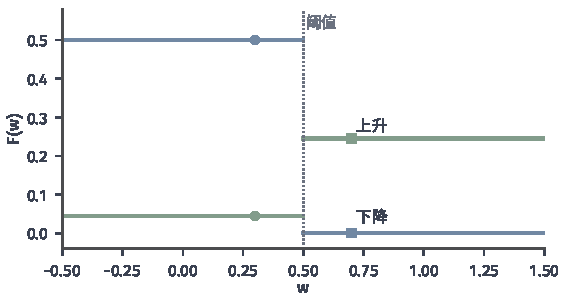
\includegraphics[width=96mm]{figures/05-optimization/05-stochastic-optimization/matplotlib/sgdb-ste-round/figure.pdf}
  \caption{取整前向上的直通更新。蓝线$F(w)=\frac12(Q(w)-1)^2$，绿线$F(w)=\frac12(Q(w)-0.3)^2$，都是分段常数，点线是取整阈值$w=0.5$。圆点是起点$w=0.3$，方块是走一步后的$w=0.7$：蓝色的损失由$0.5$降到$0$，绿色的损失由$0.045$升到$0.245$。}
  \label{fig:sgdb-ste-round}
\end{BookInlineFigure}

\paragraph{替代方向的地位}
替代方向既不是原目标的经典梯度，一般也不是凸次梯度。以$a=1$，$w=0.3$为例，若$s$是全局次梯度，要求不等式$F(y)\geq F(0.3)+s(y-0.3)$对一切$y$成立。

取$y=0.7$，得到$0\geq0.5+0.4s$，即$s\leq-1.25$。取$y=-0.4$，$F(-0.4)=0.5$，得到$s\geq0$。两者矛盾，这样的$s$不存在，$F$在该点没有全局次梯度，$-1$更不是。局部上$F$在该点附近为常数，局部的次梯度只有$0$，也不是$-1$。

所以使用替代方向的算法，只能回到实际的前向目标上评价。比较的量应是前向损失或原问题的目标值，停止准则也应基于前向量，而不是替代方向的范数是否变小。
